\documentclass{./springer/svjour3}
\usepackage{graphicx} % This lets you include figures
\graphicspath{ {./figures/} }
\usepackage[rightcaption]{sidecap}
% \usepackage{subcaption}
\usepackage{wrapfig}
\usepackage{float}
\usepackage{imakeidx}
\usepackage{comment}
\usepackage{commath}
\usepackage[titletoc]{appendix}
\usepackage{graphicx}
\usepackage{resizegather}
\usepackage[english]{babel}
% \usepackage{subcaption}
\usepackage{tabu}
\usepackage{booktabs}
\usepackage{xfrac}
\usepackage{tabularx}
% \usepackage{amssymb}
\usepackage{amsmath}
% \usepackage{amsthm}
\usepackage{commath}
\usepackage{graphicx,bm}
\usepackage{verbatim}
% \usepackage{caption}
\usepackage{lscape}
\usepackage{relsize}
\usepackage{enumitem}
\usepackage{textcomp}
\usepackage{breqn}
\usepackage{makecell}
\usepackage{longtable,tabularx}
\usepackage{multirow}
\usepackage{doi}
\usepackage{fancyhdr}
\usepackage{algorithm}
\usepackage{algpseudocode}
\usepackage{setspace}
\usepackage{footnote}
\PassOptionsToPackage{hyphens}{url}
\usepackage{hyperref}
\hypersetup{colorlinks,linkcolor={blue},citecolor={blue},urlcolor={blue}}
\usepackage[numbers]{natbib}
\usepackage{mathtools}
%\usepackage[disable]{todonotes}
\usepackage[framemethod=tikz]{mdframed}
\usepackage{booktabs,xcolor,siunitx}
\usepackage{soul}
% \usepackage{cleveref}
\usepackage[small, compact]{titlesec}
\usepackage{xcolor}
\usepackage{appendix}

% \usepackage{geometry}
% \geometry{
% a4paper,
% total={170mm,257mm},
% left=20mm,
% top=20mm,
% }

% \newtheorem{theorem}{Theorem}[section]
% \newtheorem{lemma}[theorem]{Lemma}
\newcommand{\ra}[1]{\renewcommand{\arraystretch}{#1}}
\newcommand{\degree}{\ensuremath{^\circ\,}}
\newcommand{\overbar}[1]{\mkern 1.5mu\overline{\mkern-1.5mu#1\mkern-1.5mu}\mkern 1.5mu}
\newcommand{\f}[2]{\frac{#1}{#2}}
\newcommand{\mb}[1]{\mathbf{#1}}
\newcommand{\tr}[1]{\mathrm{Tr}\left({#1}\right)}
\newcommand{\mbg}[1]{\boldsymbol{\mathbf{#1}}}
\DeclarePairedDelimiter{\ceil}{\lceil}{\rceil}
\DeclareMathAlphabet\mathbfcal{OMS}{cmsy}{b}{n}
\renewcommand{\d}{\mathop{}\!\mathrm{d}} % total derivative
\newcommand{\p}{\partial}

%\usepackage[section]{placeins}


\title{Summary of Fall 24 Research}
\author{Max Howell}
\institute{University Of Tennessee Knoxville$^*$ ($^*$corresponding author),
          \email{mhowel30@vols.utk.edu} \\
        \\
          \at MABE, University of Tennessee, Knoxville,
          \at Nathan W. Dougherty Engineering Building, 1512 Middle Dr, Knoxville, TN 37916\\
}

\date{\today}


\begin{document}
\maketitle{}
\bibliographystyle{ieeetr}
\begin{abstract}

fdas

\end{abstract}

\section{Introduction}

Control Co-Design (CCD) is an engineering design strategy used to optimize the design of a system with control in mind. CCD can be acheived using various control schemes, 
including open loop control [1], PID control, and other optimal control methods such as LQR or MPC Control. CCD has a very wide range of applications such as in 
aerospace systems [2] and in thermal energy storage [3]. While CCD has been used in various industries there has yet to be a compreherensive tool developed
to preform robust CCD using differentiable optimal control strategies such as nonlinear MPC control.

This research focuses on developing a tool which can be used in order to preform robust CCD using MPC control. This research is primarly focused on robotic applications and uses 
the MuJoCo [4] physics simulation engine in order to simulate the robotic systems. In this paper, do-mpc [5], a library for nonlinear MPC control, is used to simplify the 
implementation of MPC control. This research builds off of previous work [6] which used the Dymos Optimal Control library [7] in order to preform CCD of a simple 
two legged walking robot known as the compass gait. 

This portion of research can be broken down into three phases; phase one involved using the work done in [6] and implementing MPC control on a slightly 
more complicated three link walker. The purpose of this phase was to understand how to implement MPC control on a simplified model of a robotic system.
Phase two of this research consisted of using the knowledge of MPC control from phase one and implementing it in a more complex system using the MuJoCo physics engine.
Phase three consists of using the MPC controlled MuJoCo system and preforming CCD on the system as well as implementing more complex algorithms used in robotics such as 
path planning and obstacle avoidance. Phase three of this research is incomplete and is only discussed as a future work in this paper.

\section{Methods}

\subsection{Phase I: MPC of the Three Link Walker}

Phase I consisted of building on the research done in [6] and implementing MPC control a slightly more complex three link walker.
The compass gait is a simple two legged walking robot which is able to passively walk down an incline with no control input. The three link walker is a similar system 
but is more realistic as it uses a knee joint to walk. The compass gait as well as three link walker are hybrid systems, meaning they change dynamics based on the state of the system.
The compass gait is shown in Figure \ref{fig:compass_gait}; for a more detailed look at the dynamics of the compass gait, see [6].

\begin{figure}[!h]
  \centering
  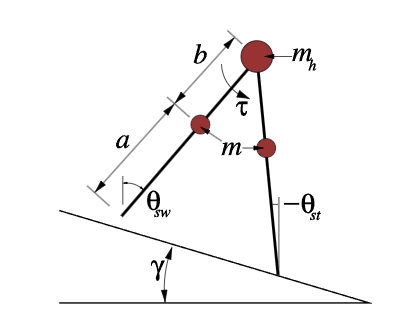
\includegraphics[width=8cm]{./figures/compassgaitmodel.png}
  \caption{Schematic of the compass gait model. Angles $\theta_{sw}$ and $\theta_{st}$ are shown as the swing leg angle and stance leg angle, respectively.}
  \label{fig:compass_gait}
\end{figure}

The three link walker system is shown in Figure \ref{fig:threeleg}. For a more detailed look at the dynamics of the three link walker, see [8]. In both the three link walker and
compass gait, there is a single control input applied to the hip.

\begin{figure}[!h]
  \centering
  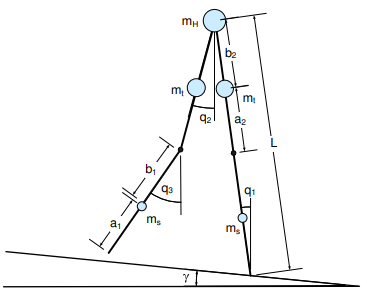
\includegraphics[width=8cm]{./figures/threeleg.png}
  \caption{Diagram of the three link walker model where q1, q2, and q3 are the stance, swing, and knee joint angles.}
  \label{fig:threeleg}
\end{figure}

MPC control was implemented on the three link walker by considering two phases for this system, a two link and a 
three link phase, where the two link phase has the same dynamics as the compass gait. A diagram showing these phases is shown in 
Figure \ref{fig:threelegstates}. These phases were treated as seperate systems with different governing equations and 
each phase was controlled using a seperate MPC controller. The transition between the two phases was triggered by "knee-strike", where the 
knee joint angle became equal to the angle of the swing leg, and "heel-strike", where the swing leg comes into contact with the ground. The 
transition between the phases were calculated using the transition equations from [8].
\begin{figure}[!h]
  \centering
  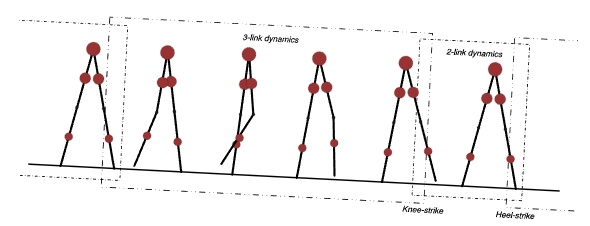
\includegraphics[width=8cm]{./figures/threelegstates.png}
  \caption{Diagram showing the two link and three link phases of the three link walker.}
  \label{fig:threelegstates}
\end{figure}

The optimization problem for the three link phase is shown in \ref{eq:threelinkphaseopt} where the states of the system ($x$) consist of 
the stance, swing, and knee joint angles as well as the angular velocities of these joints. The optimization problem for the the two link phase is 
shown in \ref{eq:twolinkphaseopt} where the states of the system ($x$) consist of the stance and swing leg angles as well as the angular velocities of these joints.

\begin{equation}
  \begin{aligned}
  &\text{Objective: $arg min_{x_k,u_k} (x_N - x_r)^TQ_N(x_N - x_r) + \sum_{k = 0}^{N-1} (x_k - x_r)^TQ(x_k - x_r) + u_k^TRu_k $}\\
  &\text{Subject to:}\\
  &\text{Control Range: $-3 < tau < 3$}\\
  &\text{Dynamic Equations of Three Link Phase}\\
  &\text{State Constraints: $x_2 > x_3 $}
  \end{aligned}
  \label{eq:threelinkphaseopt}
\end{equation}

\begin{equation}
  \begin{aligned}
  &\text{Objective: $arg min_{x_k,u_k} (x_N - x_r)^TQ_N(x_N - x_r) + \sum_{k = 0}^{N-1} (x_k - x_r)^TQ(x_k - x_r) + u_k^TRu_k $}\\
  &\text{Subject to:}\\
  &\text{Control Range: $-3 < tau < 3$}\\
  &\text{Dynamic Equations of Two Link Phase}\\
  &\text{State Constraints: $x_2 = x_3, \dot{x_2} = \dot{x_3}$}
  \end{aligned}
  \label{eq:twolinkphaseopt}
\end{equation}

In the optimization problem, $x_N$ and $x_k$ represent the terminal and current states of the system and $x_r$ respresents the target states.
$N$ is defined as the finite horizon of the MPC problem as can be thought of as how many timesteps in the future the model predicts the behavior of the system.
the $Q_N$ and $Q$ matrices are weighting matrices for the control of each state; In this case, they are equal to the identity matrix.
The $R$ matrix is a weighting matrix to penalize the control input and is equal to 1 (scalar for one control input).
The target states for each phase are the states which were pre-determined to be the knee strike and heel strike states and are shown in Table \ref{tab:threelegterm}.

\begin{table}[h]
  \centering
  \caption{Target states during MPC control of the three link walker.}
  \begin{tabular}{lrr}
  \toprule
  State & Knee Strike Target & Heel Strike Target\\
  \midrule
  $x_{sw}$ & -.106  & -0.29\\
  $x_{st}$ & 0.326 & 0.19\\
  $x_{knee}$ & 0.326 & -0.19\\
  \end{tabular}
  \label{tab:threelegterm}
\end{table}

\subsection{Phase II: MuJoCo MPC}
Phase II of this research consisted of using the knowledge of MPC which was gained from phase I and applying it to a more complex system in the MuJoCo physics engine which can 
simulate complicated robotic systems such as the humanoid shown in Figure \ref{fig:humanoid}. Instead of applying MPC control to the humanoid, MPC control was first applied to a simpler system 
in a way which can be easily scaled up to the humanoid. The chosen system was the classic cart pole control problem, where a pole with a 
mass attatched to the end is attatched to a cart which can move back and forth in one direction. This is shown in Figure \ref{fig:cartpole}. The goal of this problem is to 
control the pole to balance upright on the cart when the cart is at a stationary set location. This is done by applying a force to the cart to move it in the positive or 
negative x direction.

\begin{figure}[!h]
  \centering
  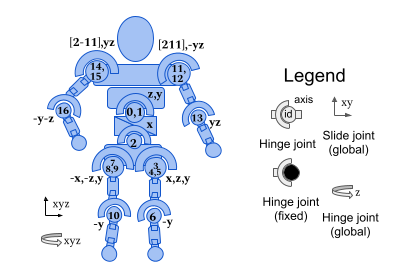
\includegraphics[width=8cm]{./figures/humanoid.png}
  \caption{Example of a humanoid robot which can be simulated in the MuJoCo physics engine.}
  \label{fig:humanoid} 
\end{figure}

\begin{figure}[!h]
  \centering
  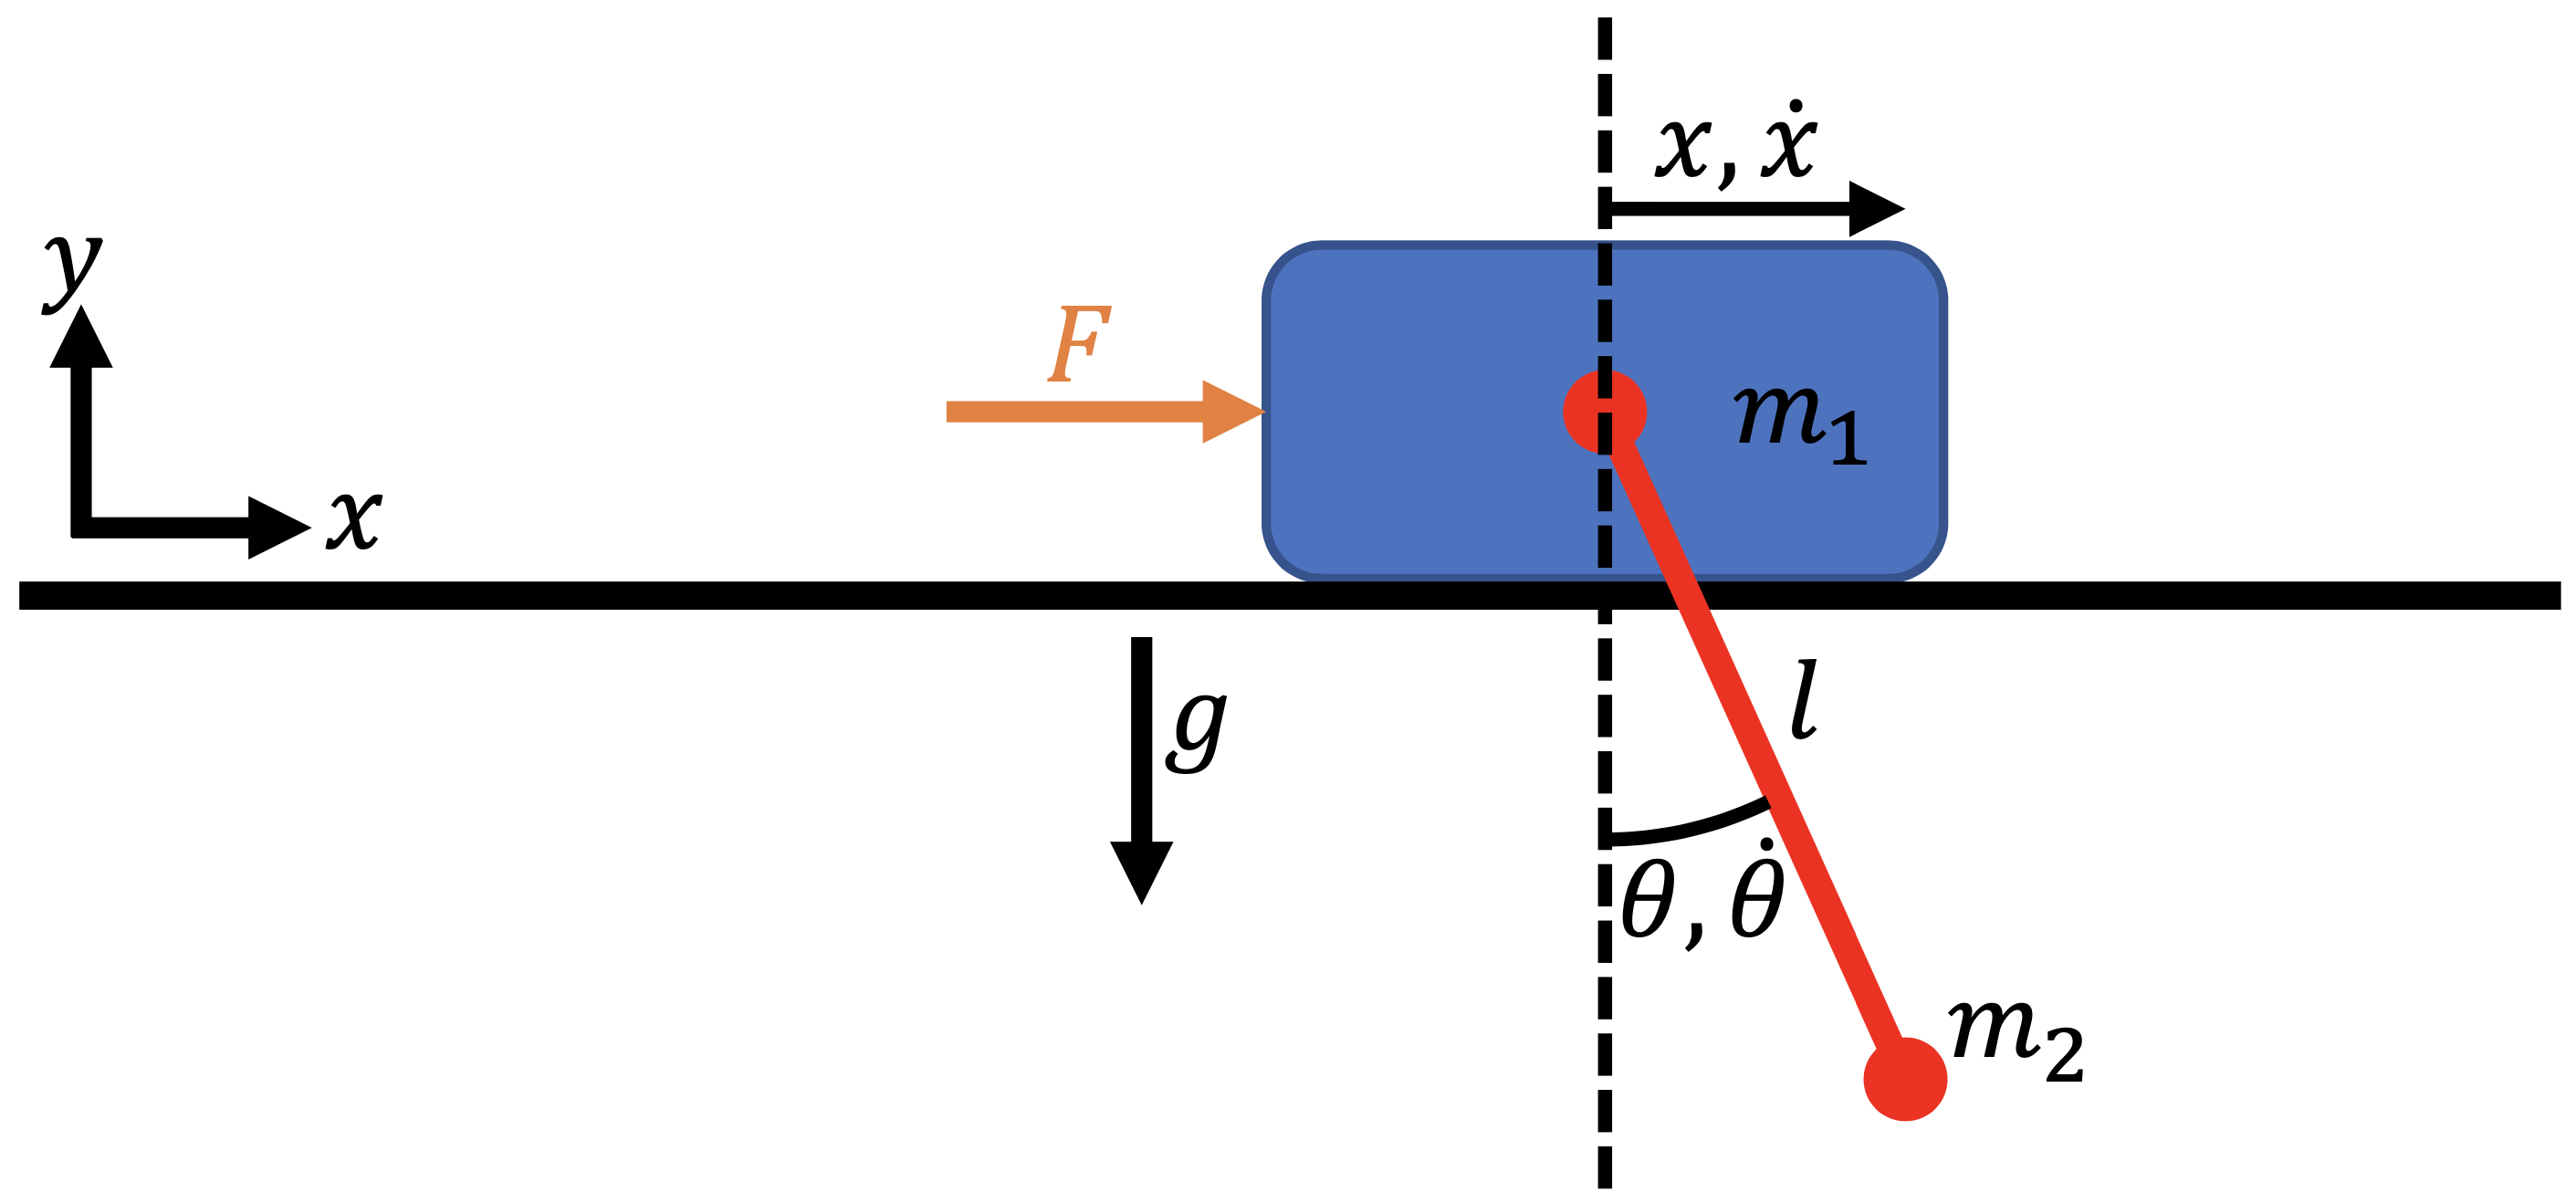
\includegraphics[width=8cm]{./figures/cartpole-dynamics.png}
  \caption{Diagram of the cart pole system.}
  \label{fig:cartpole} 
\end{figure}

The cart pole system has previously been solved with various control techniques using the governing equations of motion for the system. The equations are derived in [9]. In this
paper, the cart pole problem was solved using both MPC control with the equations of motion and using MPC control in MuJoCo in order to compare the results.
The states for each cart pole problem are shown in \ref{eq:cartpolestates} and the initial and target states of this problem are shown in
\ref{tab:init_tar_carteqn}.

\begin{equation}
  \mb{x} = 
  \begin{bmatrix}
  \\x\\
  \\\theta\\
  \\\dot{x}\\
  \\\dot{\theta}\\
  \end{bmatrix}, \quad
  \label{eq:cartpolestates}
\end{equation}

\begin{table}[h]
  \centering
  \caption{Initial and Target States of the Cart Pole Problem.}
  \begin{tabular}{lrr}
  \toprule
  State & Initial & Target\\
  \midrule
  $x$ & 0  & 0\\
  $\theta$ & 0 & $\pi$ \\
  $\dot{x}$ & 0 & 0\\
  $\dot{\theta}$ & 0 & 0\\
  \end{tabular}
  \label{tab:init_tar_carteqn}
\end{table}

Both methods of solving the cart pole problem used a similar optimization problem as shown in \ref{eq:cartpoleopt}. 
Solving the cart pole problem using the equations of motion was straight forward as the equations of motion were well known and could be easily implemented in do-mpc.
However, solving the cart pole problem in MuJoCo required a different approach in order to obtain the equations of motion for the states as the equations of motion 
were assumed to be unknown as they would be in the case of a humanoid robot or other complex system.

\begin{equation}
  \begin{aligned}
  &\text{Objective: $arg min_{x_k,u_k} (x_N - x_r)^TQ_N(x_N - x_r) + \sum_{k = 0}^{N-1} (x_k - x_r)^TQ(x_k - x_r) + u_k^TRu_k $}\\
  &\text{Subject to:}\\
  &\text{Control Range: $-35 < F < 35$}\\
  &\text{Equations of motion for respective method}\\
  &\text{State Constraints: $-3.5 < x < 3.5$}
  \end{aligned}
  \label{eq:cartpoleopt}
\end{equation}

In order to obtain the equations of motion for the MuJoCo cart pole system, a finite difference approach was used in order to solve for the linearized equations of motion at 
each time step in the simulation. These equations took the form of \ref{eq:mj_eqn_form}, where the A and B matrices were equal to the jacobian of the system 
with respect to the states and 
control, respectively.

\begin{equation}
  \dot{x} = Ax + Bu
  \label{eq:mj_eqn_form}
\end{equation}

The A and B matrices were found using the finite difference method by first obtaining the nominal (current, found from MuJoCo simulation)
state of the system as denoted in \ref{eq:nomstate}
and then perturbing each state one at a time as shown in \ref{eq:pertA} (repeat for all columns of the square matrix A) where $\epsilon$
is a small number in order to obtain the A matrix. The B matrix was 
obtained in a similar manner by perturbing the control input as shown in \ref{eq:pertB}.

\begin{equation}
  x_{nom} = f(x^0, \theta^0, \dot{x}^0, \dot{\theta}^0, F^0)
  \label{eq:nomstate}
\end{equation}

\begin{equation}
  A \text{ (Column One)} =\frac{ f(x^0 + \epsilon, \theta^0, \dot{x}^0, \dot{\theta}^0, F^0) - f(x^0, \theta^0, \dot{x}^0, \dot{\theta}^0, F^0)}{\epsilon}
  \label{eq:pertA}
\end{equation}

\begin{equation}
  B =\frac{ f(x^0, \theta^0, \dot{x}^0, \dot{\theta}^0, F^0 + \epsilon) - f(x^0, \theta^0, \dot{x}^0, \dot{\theta}^0, F^0)}{\epsilon}
  \label{eq:pertB}
\end{equation}

After determining the A and B matrices for the cart pole MuJoCo system, the problem could then be solved by integrating the MuJoCo engine with the do-mpc interface.
However, since the A and B matrices were being calculated at each time step, the dompc problem needed to be re-initialzed at each time step with the updated A and B matrices.
This caused computational inefficency and will be addressed in future research.

\section{Results}

\subsection{Phase I: MPC of the Three Link Walker}

The three link walker was simulated using the MPC control scheme outlined in the previous section. The 
walker was also simulated without control in order to compare the limit cycles of the simulations. The parameters used for simulation are shown in Table
\ref{tab:walker_params} and the initial condition is shown in Table \ref{tab:walker_init}
The gait of the passive walker as well as 
the timeseries states are shown in Figure \ref{fig:passive_sol}. As can be seen, both the knee strike and heel strike can be seen clearly in the gait cycle.
The knee strike occurs as a small instantanious change in angular velocity of the swing leg (the $x_2, x_5$ leg). The heel strike occurs when the system switches the swing legs 
and the stance legs. This can be seem as the transition from the $x_2, x_5$ graph to the $x_1, x_4$ graph.

\begin{table}[h]
  \centering
  \caption{Parameters of the Three Link Walker Used in Simulation.}
  \begin{tabular}{lr}
  \toprule
  Parameter & Knee Strike Target\\
  \midrule
  $a_1$ & 0.375\\
  $b_1$ & 0.125\\
  $a_2$ & 0.175\\
  $b_2$ & 0.325\\
  $m_h$ & 0.5\\
  $m_t$ & 0.5\\
  $m_s$ & 0.05\\
  $\gamma$ & 0.05\\
  \end{tabular}
  \label{tab:walker_params}
\end{table}

\begin{table}[h]
  \centering
  \caption{Initial Condition of the three link walker.}
  \begin{tabular}{lrr}
  \toprule
  State & Initial Condition\\
  \midrule
  $x_{1}$ & 0.1877 \\
  $x_{2}$ & -0.2884\\
  $x_{3}$ & -0.2884\\
  $x_{4}$ & -1.1014\\
  $x_{5}$ & -0.0399\\
  $x_{6}$ & -0.0399\\
  \end{tabular}
  \label{tab:walker_init}
\end{table}

\begin{figure}[!h]
  \centering
  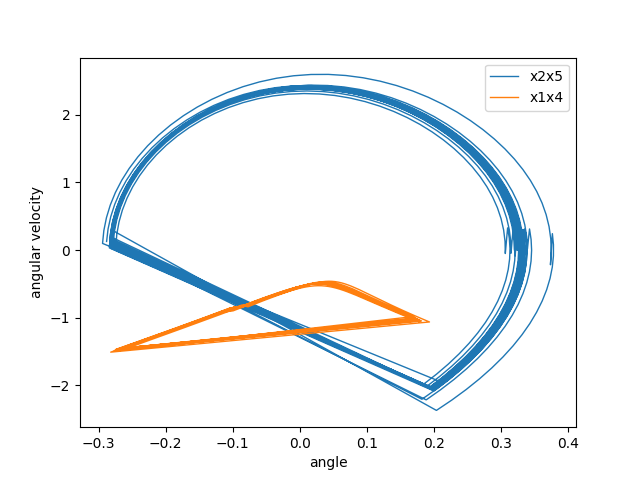
\includegraphics[width=.4\linewidth]{./figures/gait_passive.png} % Just stack two includegraphics!
  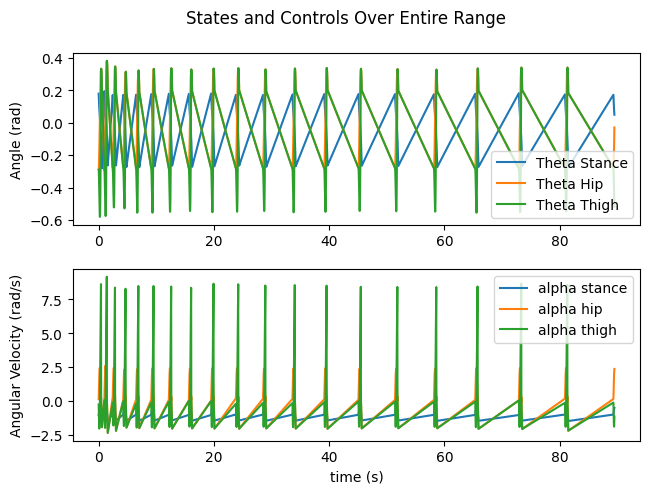
\includegraphics[width=.4\linewidth]{./figures/ts_passive.png}
  \caption{The Gait cycle and timeseries states of the passive three link walker}
  \label{fig:passive_sol}
  \end{figure}

The MPC controlled graphs for the three link walker are similarly shown in Figure \ref{fig:active_sol}. The chaotic nature of the gait cycle in the active three link walker 
can be clearly seen. Despite the walker acheiving the goal of not falling over, there are clear stability issues with the MPC controller. This is most likely due 
to the way the objective of control is defined. Since the target states are simply defined as predetermined states where knee strike and heel strike occur, the 
active walker is constrained in its motion and is unable to find a stable gait cycle which passes through the specified transition points. 
Using a different control objective such as controlling the average forward speed of the walker or doing path planning to find the optimal path the legs should take 
would most likely cause the gait cycle of this walker to be stable.

\begin{figure}[!h]
  \centering
  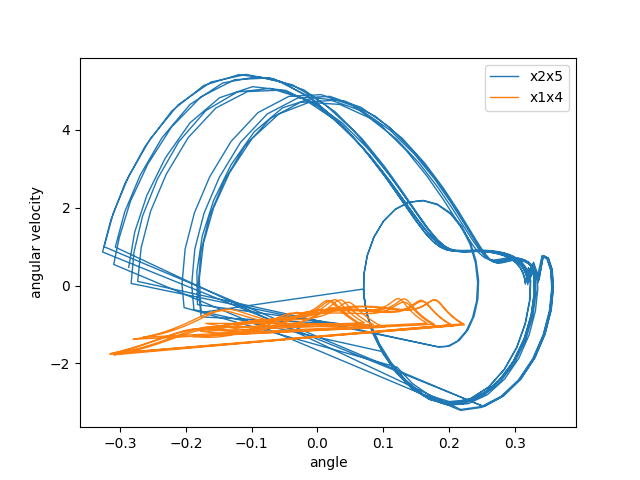
\includegraphics[width=.4\linewidth]{./figures/three_gait.png} % Just stack two includegraphics!
  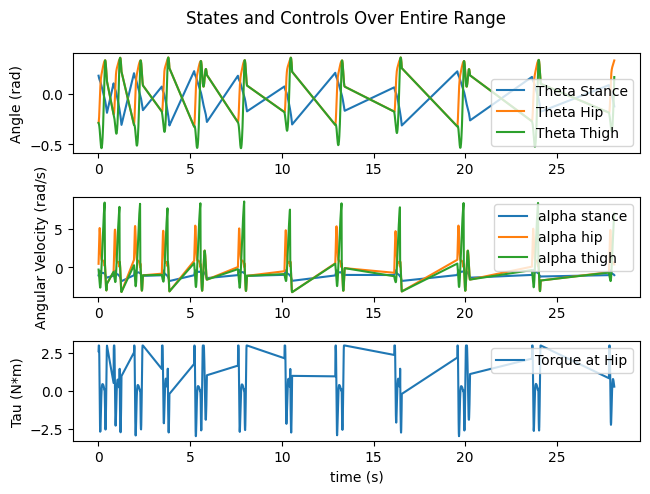
\includegraphics[width=.4\linewidth]{./figures/timeseries_data.png}
  \caption{The Gait cycle and timeseries states of the active three link walker}
  \label{fig:active_sol}
\end{figure}

\subsection{MuJoCo MPC}
The cartpole system was simulated using MPC control for both cases, using the equations of motion and MuJoCo. The parameters for the cartpole using the equations of motion are shown 
in Table \ref{tab:cartpole_params}. The MuJoCo case used the same pole length and cart mass; however, it should be noted that the physics of the system were slightly different.
In the MuJoCo system, the pole was treated as a solid rod of constant density, while in the equations of motion case, the pole was treated as a massless rod 
with a point mass attatched to the top of it. This changes the dynamics of the system and should be addressed in future research.

\begin{table}[h]
  \centering
  \caption{Parameters Used in the Cart Pole Simulation (Eqs of Motion)}
  \begin{tabular}{lrr}
  \toprule
  Parameter & Value\\
  \midrule
  Cart mass & 0.6 \\
  Pole mass & 0.2\\
  Pole Length & 0.5\\
  \end{tabular}
  \label{tab:cartpole_params}
\end{table}

The timeseries solution of the equations of motion case is shown in Figure \ref{fig:sol_eqn}. As can be seen, the system reaches a steady state with the pole balanced 
at the upright position and the cart at the target state. The timeseries solution of the MuJoCo case is shown in Figure \ref{fig:sol_mj}. In the MuJoCo case, it can 
also be seen that the pole is balanced in the upright position at the end of the simulation with the cart in the target state (in the MuJoCo system, the 
$\theta$ axis is offset by $\pi$, meaning the target and initial states are switched). It can also be seen that the MuJoCo controller uses more total force to 
balance the cartpole and takes a longer time to reach steady state. This is most likely due to the difference in physics between the two systems and will be addressed in the future.

\begin{figure}[!h]
  \centering
  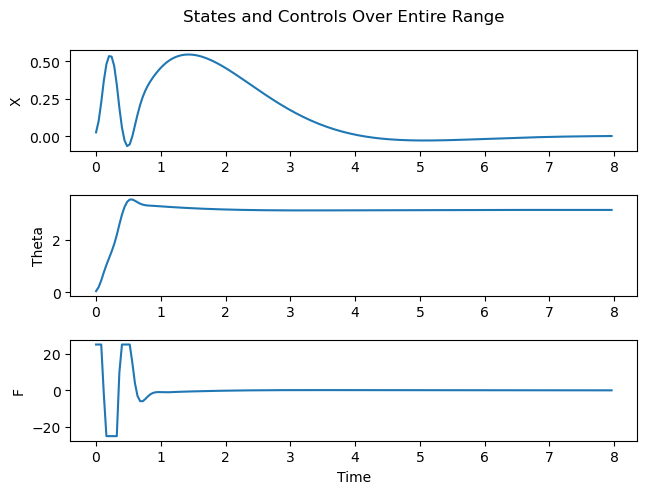
\includegraphics[width=8cm]{./figures/timeseries_dynamics.png} % Just stack two includegraphics!
  \caption{The timeseries solution to the cartpole problem (using equations of motion)}
  \label{fig:sol_eqn}
\end{figure}

\begin{figure}[!h]
  \centering
  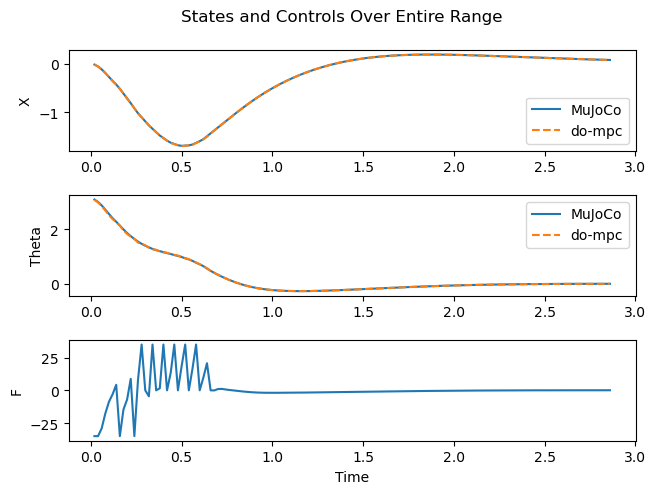
\includegraphics[width=8cm]{./figures/cartpole_mj_timeseries_normlen.png} % Just stack two includegraphics!
  \caption{The timeseries solution to the cartpole using MuJoCo}
  \label{fig:sol_mj}
\end{figure}

In Figure \ref{fig:sol_mj} the calculated states from the MuJoCo simulation and the states from the linearized equations of motion (using 
finite difference) are compared. As can be seen the MuJoCo states are equal to the linearized equations of motion states (do-mpc states) throughout the duration 
of the simulation. One thing that should be considered however, is that when using MPC control, the future states of the system are predicted for a set 
"control horizon" (70 time steps in this case). Since the system is linearized at each time step during the simulation, it is expected that the current state of the 
system is equivelant between the MuJoCo simulation and the linearized equations of motion; however, during the control horizon it is probable that after a certain amount of time 
when the state of the system is sufficently far from the state about which the system was linearized that the predictions become inaccurate. This means that it is possible 
for a control horizon which is too long to cause the control to fail due to the inaccuracy in the future predictions of the model.

While the MPC controller works to stabilize the MuJoCo system when the parameters are the same as the above case, it was observed 
that if the parameters are changed too far from the original parameters the control will fail. An example of this using the parameters shown in 
\ref{tab:fail_cartpole} is shown in Figure \ref{fig:fail_cartpole}. As can be seen, the pole position is unstable and does not balance. It is hypothesied that 
this failure is caused by the difference in physics between the two cases, as the equations of motion case does not fail when the parameters are changed. It is also possible 
that the inaccurate control horizon is causing this failure. This is being investigated by creating a new MuJoCo model which is exactly the same as the equations of motion case 
and comparing the two cases again.


\end{document}
